\documentclass[12pt]{article}
\usepackage[brazil]{babel}
\usepackage{graphicx}
\usepackage{mathtools}
\usepackage{float} 
\usepackage{xcolor}
\usepackage{amsmath, amssymb, bm}


\usepackage{array}
\usepackage{booktabs}



% margenes
\usepackage[a4paper,left=3cm,right=3cm,top=3cm]{geometry}

%opening
\title{}
\author{}

\begin{document}

\begin{center}
	{\tiny {\normalsize {\large \textbf{Convecção}\\ Lista de exercicios 5\\
	
	\textbf{Cristian Herledy Lopez Lara}}}}
\end{center}

\subsection*{Problema 7.12 livro texto}

\begin{figure}[H]
	\centering
	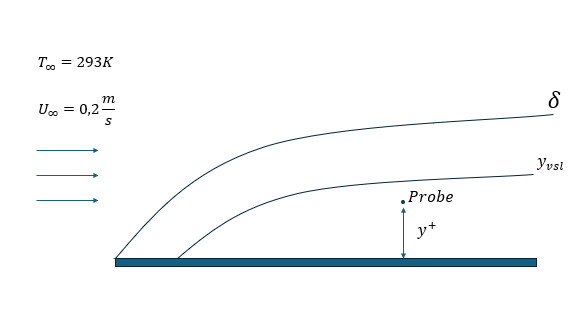
\includegraphics[width=.65\textwidth]{Figures/1_1}
	\caption{Escoamento da camada limite com sensor de medição em $y^+$}
\end{figure}

\textbf{Desenvolvimento} 

A análise começa com a transformação das equações de conservação em equações médias temporais. Começamos com a transformação:

\begin{equation}
	u = \overline{u} + u', \quad v = \overline{v} + v'
\end{equation}

\begin{equation}
	P = \overline{P} + P', \quad T = \overline{T} + T'
\end{equation}

Onde com essas variáveis temos para massa, momento e energia

\begin{equation}
	\frac{\partial \overline{u}}{\partial x} + \frac{\partial \overline{v}}{\partial y} = 0
\end{equation}

\begin{equation}
	\overline{u} \frac{\partial \overline{u}}{\partial x} + \overline{v} \frac{\partial \overline{u}}{\partial y}   = - \frac{1}{\rho} \frac{\partial \overline{P}}{\partial x} + \nu \nabla^2 \overline{u} - \frac{\partial}{\partial x} \left( \overline{u'v'} \right) - \frac{\partial}{\partial y} \left( \overline{u'w'} \right)
\end{equation}

\begin{equation}
	\overline{u} \frac{\partial \overline{v}}{\partial x} + \overline{v} \frac{\partial \overline{v}}{\partial y}  = - \frac{1}{\rho} \frac{\partial \overline{P}}{\partial y} + \nu \nabla^2 \overline{v} - \frac{\partial}{\partial x} \left( \overline{u'v'} \right) - \frac{\partial}{\partial y} \left( \overline{v'v'} \right) 
\end{equation}

\begin{equation}
	\overline{u} \frac{\partial \overline{T}}{\partial x} + \overline{v} \frac{\partial \overline{T}}{\partial y} = \alpha \nabla^2 \overline{T} - \frac{\partial}{\partial x} \left( \overline{u'T'} \right) - \frac{\partial}{\partial y} \left( \overline{v'T'} \right)
\end{equation}

A partir dessas equações, por meio de várias simplificações do Capítulo 2 e suposições adicionais, serão fornecidas as equações que regem a camada limite.
As equações de momento e energia em x para esta região são dadas por

\begin{equation}
	\overline{u} \frac{\partial \overline{u}}{\partial x} + \overline{v} \frac{\partial \overline{u}}{\partial y} = - \frac{1}{\rho} \frac{\partial \overline{P}}{\partial x} + \frac{1}{\rho} \frac{\partial}{\partial y} \left( \mu \frac{\partial \overline{u}}{\partial y} - \rho u'v' \right)
\end{equation}

\begin{equation}
	\overline{u} \frac{\partial \overline{T}}{\partial x} + \overline{v} \frac{\partial \overline{T}}{\partial y} = \frac{1}{\rho c_p} \frac{\partial}{\partial y} \left( k \frac{\partial \overline{T}}{\partial y} - \rho c_p v' T' \right)
\end{equation}

Onde as novas expressões junto os termos difusivos estão relacionadas à tensão de cisalhamento turbulento e ao fluxo de calor, respectivamente.

\begin{equation}
	-\rho u'v' = \rho \epsilon_M \frac{\partial \overline{u}}{\partial y}
\end{equation}

\begin{equation}
	-\rho c_p v' T' = \rho c_p \epsilon_H \frac{\partial \overline{T}}{\partial y} 
\end{equation}

Esses termos adicionais estão associados à tensão de cisalhamento  e ao fluxo de calor aparentes. Com essas expressões, as equações de momento em x e energia serão

\begin{equation}
	\overline{u} \frac{\partial \overline{u}}{\partial x} + \overline{v} \frac{\partial \overline{u}}{\partial y} = - \frac{1}{\rho} \frac{\partial \overline{P}}{\partial x} + \frac{\partial}{\partial y} \left[ \left( \nu + \epsilon_M \right) \frac{\partial \overline{u}}{\partial y} \right]
\end{equation}

\begin{equation}
	\overline{u} \frac{\partial \overline{T}}{\partial x} + \overline{v} \frac{\partial \overline{T}}{\partial y} = \frac{\partial}{\partial y} \left[ \left( \alpha + \epsilon_H \right) \frac{\partial \overline{T}}{\partial y} \right]
\end{equation}

\textbf{a)} Partindo do termo adimensional da coordenada espacial vertical

\begin{equation}
	y^+ = \frac{y u_*}{\nu}
\end{equation}

\begin{equation}
	u_* = \left( \frac{\tau_0}{\rho} \right)^{1/2}
\end{equation}

Onde $u*$ faz referencia a velocidade de atrito. A tensão de cisalhamento na parede é calculada com a expressão

\begin{equation}
	\frac{\tau_0}{\rho U_\infty^2} = 0.0296 \left( \frac{U_\infty x}{\nu} \right)^{-1/5}
\end{equation}

\begin{equation}
	\tau_0 =  0.0296 \left( \frac{0,2 \frac{m}{s} \cdotp 6m}{1,003 x 10^{-6}\frac{m^2}{s}} \right)^{-1/5} 998\frac{Kg}{m^3}\cdotp (0.2\frac{m}{s})^2 = 0,071 Pa
\end{equation}

\begin{equation}
	u_* = \left( \frac{19,40 \frac{Kg}{m^2s}}{ 998\frac{Kg}{m^3}} \right)^{1/2} = 8,48x10^{-3}\frac{m}{s} 
\end{equation}

\begin{equation}
	y = \frac{y^+ \nu}{u_*} = \frac{(2.7)(1,003 x 10^{-6}\frac{m^2}{s})}{0.13 \frac{m}{s}} = 3,18x10^{-4}m = 0,31mm
\end{equation}

O número de Reynolds é da ordem de $1,2 x 10^{6}$ , portanto é um escoamento turbulento.
\textbf{b)} Para o cálculo da espessura da camada limite

\begin{equation}
	\frac{\delta}{x} = 0.37 \left( \frac{U_\infty x}{\nu} \right)^{-1/5}
\end{equation}

\begin{equation}
	\delta = 0.37 \left(  \frac{0,2 \frac{m}{s} \cdotp 6m}{1,003 x 10^{-6}\frac{m^2}{s}}\right)^{-1/5}\cdotp6m = 0,13m
\end{equation}

\textbf{c)} Tomando o valor médio do número de Nusselt (eq. 7.78")

\begin{equation}
	\overline{Nu_L} = 0.037 Re_L^{4/5} Pr^{1/3} \quad (Pr \geq 0.5)
\end{equation}
\begin{equation}
	\overline{Nu_L} = 0.037 \left(  \frac{0,2 \frac{m}{s} \cdotp 6m}{1,003 x 10^{-6}\frac{m^2}{s}}\right)^{4/5} 7,02^{1/3} \quad = 6320
\end{equation}

\begin{equation}
	\overline{Nu_L} = \frac{\overline{h}L}{k}
\end{equation}
\begin{equation}
	\overline{h} = \frac{\overline{k}{Nu_L}}{L} = \frac{0,588 \frac{W}{mK}6320}{6m} = 630\frac{W}{m^{2}K}
\end{equation}

\subsection*{Problema 7.20 livro texto}

\begin{figure}[H]
	\centering
	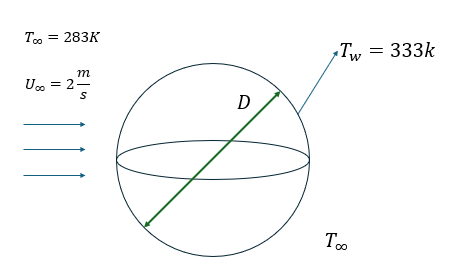
\includegraphics[width=.65\textwidth]{Figures/1_2}
	\caption{Esfera resfriada por escoamento de ar}
\end{figure}
Para este problema, serão consideradas as equações constitutivas do problema 7.12 (em coordenadas esféricas). Dadas as premissas das equações de conservação para o problema da camada limite, iniciaremos os cálculos a partir da definição do número de Reynolds.

\begin{equation}
	Re_{D} =  \frac{U_\infty D}{\nu} = \left(  \frac{2 \frac{m}{s} \cdotp 0.06m}{1,426 x 10^{-5}\frac{m^2}{s}}\right) = 8415
\end{equation}

A correlação para o valor do número médio de Nusselt é dada pela correlação da equação 7.104, para a superfície do bulbo isotérmico e escoamento livre isotérmico


\begin{equation}
	\overline{Nu_D} = 2 + \left( 0.4 Re_D^{1/2} + 0.06 Re_D^{2/3} \right) Pr^{0.4} \left( \frac{\mu_\infty}{\mu_w} \right)^{1/4}
\end{equation}


\begin{equation}
	\overline{Nu_D} = 2 + \left( 0.4 \left(  \frac{2 \frac{m}{s} \cdotp 0.06m}{1,426 x 10^{-5}\frac{m^2}{s}}\right)^{1/2} + 0.06 \left(  \frac{2 \frac{m}{s} \cdotp 0.06m}{1,426 x 10^{-5}\frac{m^2}{s}}\right)^{2/3} \right) 0,73^{0.4} \left( \frac{1,778x10^{-5}\frac{m^{2}}{s}}{2,008x10^{-5}\frac{m^{2}}{s}} \right)^{1/4}
\end{equation}

\begin{equation}
	\overline{Nu_D} =  \frac{\overline{h} D}{k}
\end{equation}

\begin{equation}
	\overline{h} = \frac{54,50 (0,024\dfrac{W}{mK})}{0,06m} = 21.8 \frac{W}{m^2}K
\end{equation}

Calculando a taxa de transferência de calor por convecção

\begin{equation}
	q = \overline{h}\Delta T A
\end{equation}


\begin{equation}
	q =  21.8 \frac{W}{m^2}K \cdotp50K \cdotp 0,011 m^{2} = 12,3 W
\end{equation}

\begin{thebibliography}{999}
	
	
	\bibitem{abejan}
	Adrian Bejan,
	Convection Heat Transfer.
	Durham, North Carolina,
	3rd Edition,
	2004.
	
	
\end{thebibliography}



\end{document}





